\documentclass[specialist, subf, href, colorlinks=true, 14pt, times, mtpro, final]{disser}

\usepackage[english, russian]{babel}
\usepackage[T2A]{fontenc}
\usepackage [utf8] {inputenc}
\usepackage{amsmath,amsthm,amssymb}
\usepackage {wrapfig}
\usepackage {enumitem}  
\usepackage{graphicx}
\usepackage{multicol}
\usepackage{mathrsfs}
\usepackage{xcolor}
\usepackage{hyperref}
\usepackage{tikz}
\usepackage{pdfpages}


\usetikzlibrary{decorations.pathreplacing}
\usepackage[noend]{algpseudocode}
\usepackage[a4paper, mag=1000, includefoot, left=3cm, right=1.5cm, top=2cm, bottom=2cm, headsep=1cm, footskip=1cm]{geometry}
\usepackage{floatrow}
\usepackage{tikz}
\usetikzlibrary{graphs}

\theoremstyle{definition}
\newtheorem{defn}{Определение}[section]
\newtheorem{example}{Пример}[section]
\newtheorem{state}{Утверждение}[section]
\newtheorem{theorem}{Теорема}[section]
\newtheorem{lemma}{Лемма}[section]
\newtheorem{axiom}{Аксиома}[section]
\newtheorem{consequence}{Следствие}[section]

\begin{document}
	\begin{titlepage}
	\begin{center}

		Федеральное государственное бюджетное образовательное учреждение высшего образования 
		<<Московский Государственный Университет им.\,М.\,В.\,Ломоносова>>\\
		
		Механико-математический факультет
		
		Кафедра вычислительной математики\\[0.6cm]
		
		\begin{figure}[!htp]
				\begin{center}
						{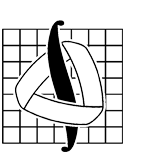
\includegraphics[width=20mm]{pics/mmlogo.png}}
					\end{center}
			\end{figure}
		
		\vspace{3cm}
			
		{\bf Численное моделирование нестационарного одномерного течения газа с использованием неявной параллельной разностной схемой с центральными разностями $(\rho, u)$}
		
		\vspace{5cm}
		\begin{flushright}
			{\bfРаботу выполнил:}\\
			студент 4 курса Сибгатуллин Артур Петрович\\[0.5cm]
		\end{flushright}
		\vspace{1cm}
		
		\normalsize Москва, 2021
	\end{center}
\end{titlepage}

	
	\tableofcontents
	\newpage
	
	\section{Введение}
\subsection{Постановка задачи}

Рассмотрим систему уравнений, описывающую нестационарное одномерное движение вязкого баротропного газа:

\begin{equation} \label{eq:task}
	\begin{cases}
		\begin{array}{l}
			\frac{\partial\rho}{\partial t} + \frac{\partial \rho u}{\partial x} = \rho f_0 \\
			\rho \frac{\partial u}{\partial t} + \rho u \frac{\partial u}{\partial x} + \frac{\partial p}{\partial x} = \mu \frac{\partial^2u}{\partial x^2} + \rho \\
			p = p(\rho)
		\end{array}
	\end{cases}
\end{equation}

Через $\mu$ обозначен коэффициент вязкости газа, который будем считать известной положительной
константой. Известными также будем считать функцию давления газа $p$ (в данной работе будем рассматривать $p(\rho) = C\rho$, где $C$ - положительная константа) и вектор внешних сил $f$. $f$ - функция переменных Эйлера: $(t, \, x) \in Q = \Omega_t \times \Omega_x = [0; \, T] \times [0; \, X]$.

Неизвестные функции: плотность $\rho$ и скорость $u$ также являются функциями переменных Эйлера.

Перепишем систему $(1)$ в эквивалентный вид, при условии того, что $\rho$ и $u$ гладкие: 

\begin{equation} \label{eq:task_reformulate}
	\begin{cases}
		\begin{array}{l}
			\frac{\partial \rho}{\partial t} + \frac{1}{2}\left(u\frac{\partial \rho}{\partial x} + \frac{\partial \rho u}{\partial x} + \rho \frac{\partial u}{\partial x}\right) = 0\\
			\frac{\partial u}{\partial t} + \frac{1}{3}\left(u\frac{\partial u}{\partial x} + \frac{\partial u^2}{\partial x}\right) +\frac{1}{\rho}\frac{\partial p}{\partial x} = \frac{\mu}{\rho}\frac{\partial^2 u}{\partial x^2} + f			
		\end{array}
	\end{cases}
\end{equation}

Система \eqref{eq:task} дополнена граничными условиями:
\begin{equation} \label{eq:terms}
	\begin{array}{lc}
		(\rho, \, u)|_{t = 0} = (\rho_0, \, u_0), &\quad x \in [0; \, X] \\
		u (t, \, 0) = u (t, \, X) = 0, &\quad t \in [0; \, T]
	\end{array}
\end{equation}

\subsection{Основные обозначения}
Введем на $\Omega_x$ и $\Omega_t$ сетки:
\begin{equation}
	\begin{array}{lc}
		\omega_x = \{mh: m = 0, \dots, M\}, h = \frac{X}{M}\\
		\omega_t = \{n\tau: n = 0, \dots, N\}, \tau = \frac{T}{N}\\
	\end{array}
\end{equation}

Для сокращения записи значение для произвольной функции f в узле $(n,m)$ сетки $\omega_x x \omega_t$ обозначим за $f_m^n$. Введем следующие обозначения:
\begin{equation}
	\begin{array}{lc}
		\hat{f} = f_m^{n+1}\\
		f_t = \frac{f_m^{n+1} - f_m^n}{\tau}\\
		f_x = \frac{f_{m+1}^n - f^n_m}{h}\\
		f_{\bar{x}} = \frac{f_m^n - f^n_{m-1}}{h}\\
		f_{\mathring{x}} = \frac{f_{m+1}^n - f^n_{m-1}}{2h}\\
		f_{x\bar{x}} = \frac{f^n_{m-1} - 2f_m^n + f^n_{m+1}}{h^2}\\
	\end{array}
\end{equation}
	
	
%%	\section{Постановка задачи}
Задачей данной работы является поддержание корректной работы с объектами \emph{Workflow} через графический интерфейс и \emph{Custom code}.


	
%%	\section{Решение задачи}
Каждый объект (\emph{Geo Data}) в проекте \emph{Geolody Designer} может быть найдем с помощью метаинформации об объекте:
\begin{itemize}
	\item \emph{Unique ID}. 64-битное беззнаковое целое число. С его помощью объекты идентифицируются в рамках одного проекта \emph{Geolody Designer}.
	\item \emph{UUID - Universally Unique IDentifier}\cite{UUID} (с англ. универсальный уникальный идентификатор). 128-битный идентификатор, уникальность которого гарантируется стандартом\cite{UUID}, даже при генерации на различных компьютерах одновременно. Необходим для индентификации между разными проектами \emph{Geolody Designer}.
	\item \emph{Absolute name} (с англ. абсолютное имя). Имя объекта с учетом всех родительских объектов проекта \emph{Geolody Designer}. Пример:  "3DСетки/Сетка1/Свойство2"\ 
	\item \emph{Unique name} (с англ. уникальное имя). Имя объекта в рамках одного пространства имен родительского объекта в проекте \emph{Geolody Designer}. Пример: пространство имен -- "3DСетки"\ , уникальное имя -- "Сетка1"\ 
\end{itemize}

Имеющийся в коде \emph{Geology Designer} умный указатель -- \emph{Geo Data pointer} может осуществлять поиск указателя к объекту по метаинформации (\emph{Unique ID, Absolute name}) о нем и обеспечивать кооректное поведение \emph{Geology Designer} даже при обращение к удаленному объекту проекта из Workflow. 

Для уменьшения накладных расходов на работу \emph{Geo Data pointer} используется кэширование. В проекте, поиск по-которому осуществляет \emph{Geo Data pointer},  хранится количество изменений (добавление нового объекта, удаление существующего объекта ...) состояния проекта, назовем это количество \emph{Mutation counter} (с англ. счетчик изменений). При обращении к объекту через \emph{Geo Data pointer} умный указатель проверяет изменился ли проект с момента последнего обновления хранящегося в нем указателя на \emph{Geo Data}, если проект изменился, то указатель обновляется.

Однако в имеющейся реализации \emph{Geo Data pointer} нельзя было использовать, так как возникали проблемы с \emph{Preloader}: невозможность работы с копроектом и отсутствие поиска по всем из указанных выше идентификаторов.

В рамках данной курсовой работы было решено переделать имеющийся \emph{Geo Data pointer} для корректной работы со всеми идентификаторами и возможности поиска объекта как в проекте, так и в копроекте, а также поддержать корректную работу методов \emph{Python}-объектов в \emph{Custom code} c новой логикой хранения объектов в Workflow.

\begin{figure}[H]	
	\center{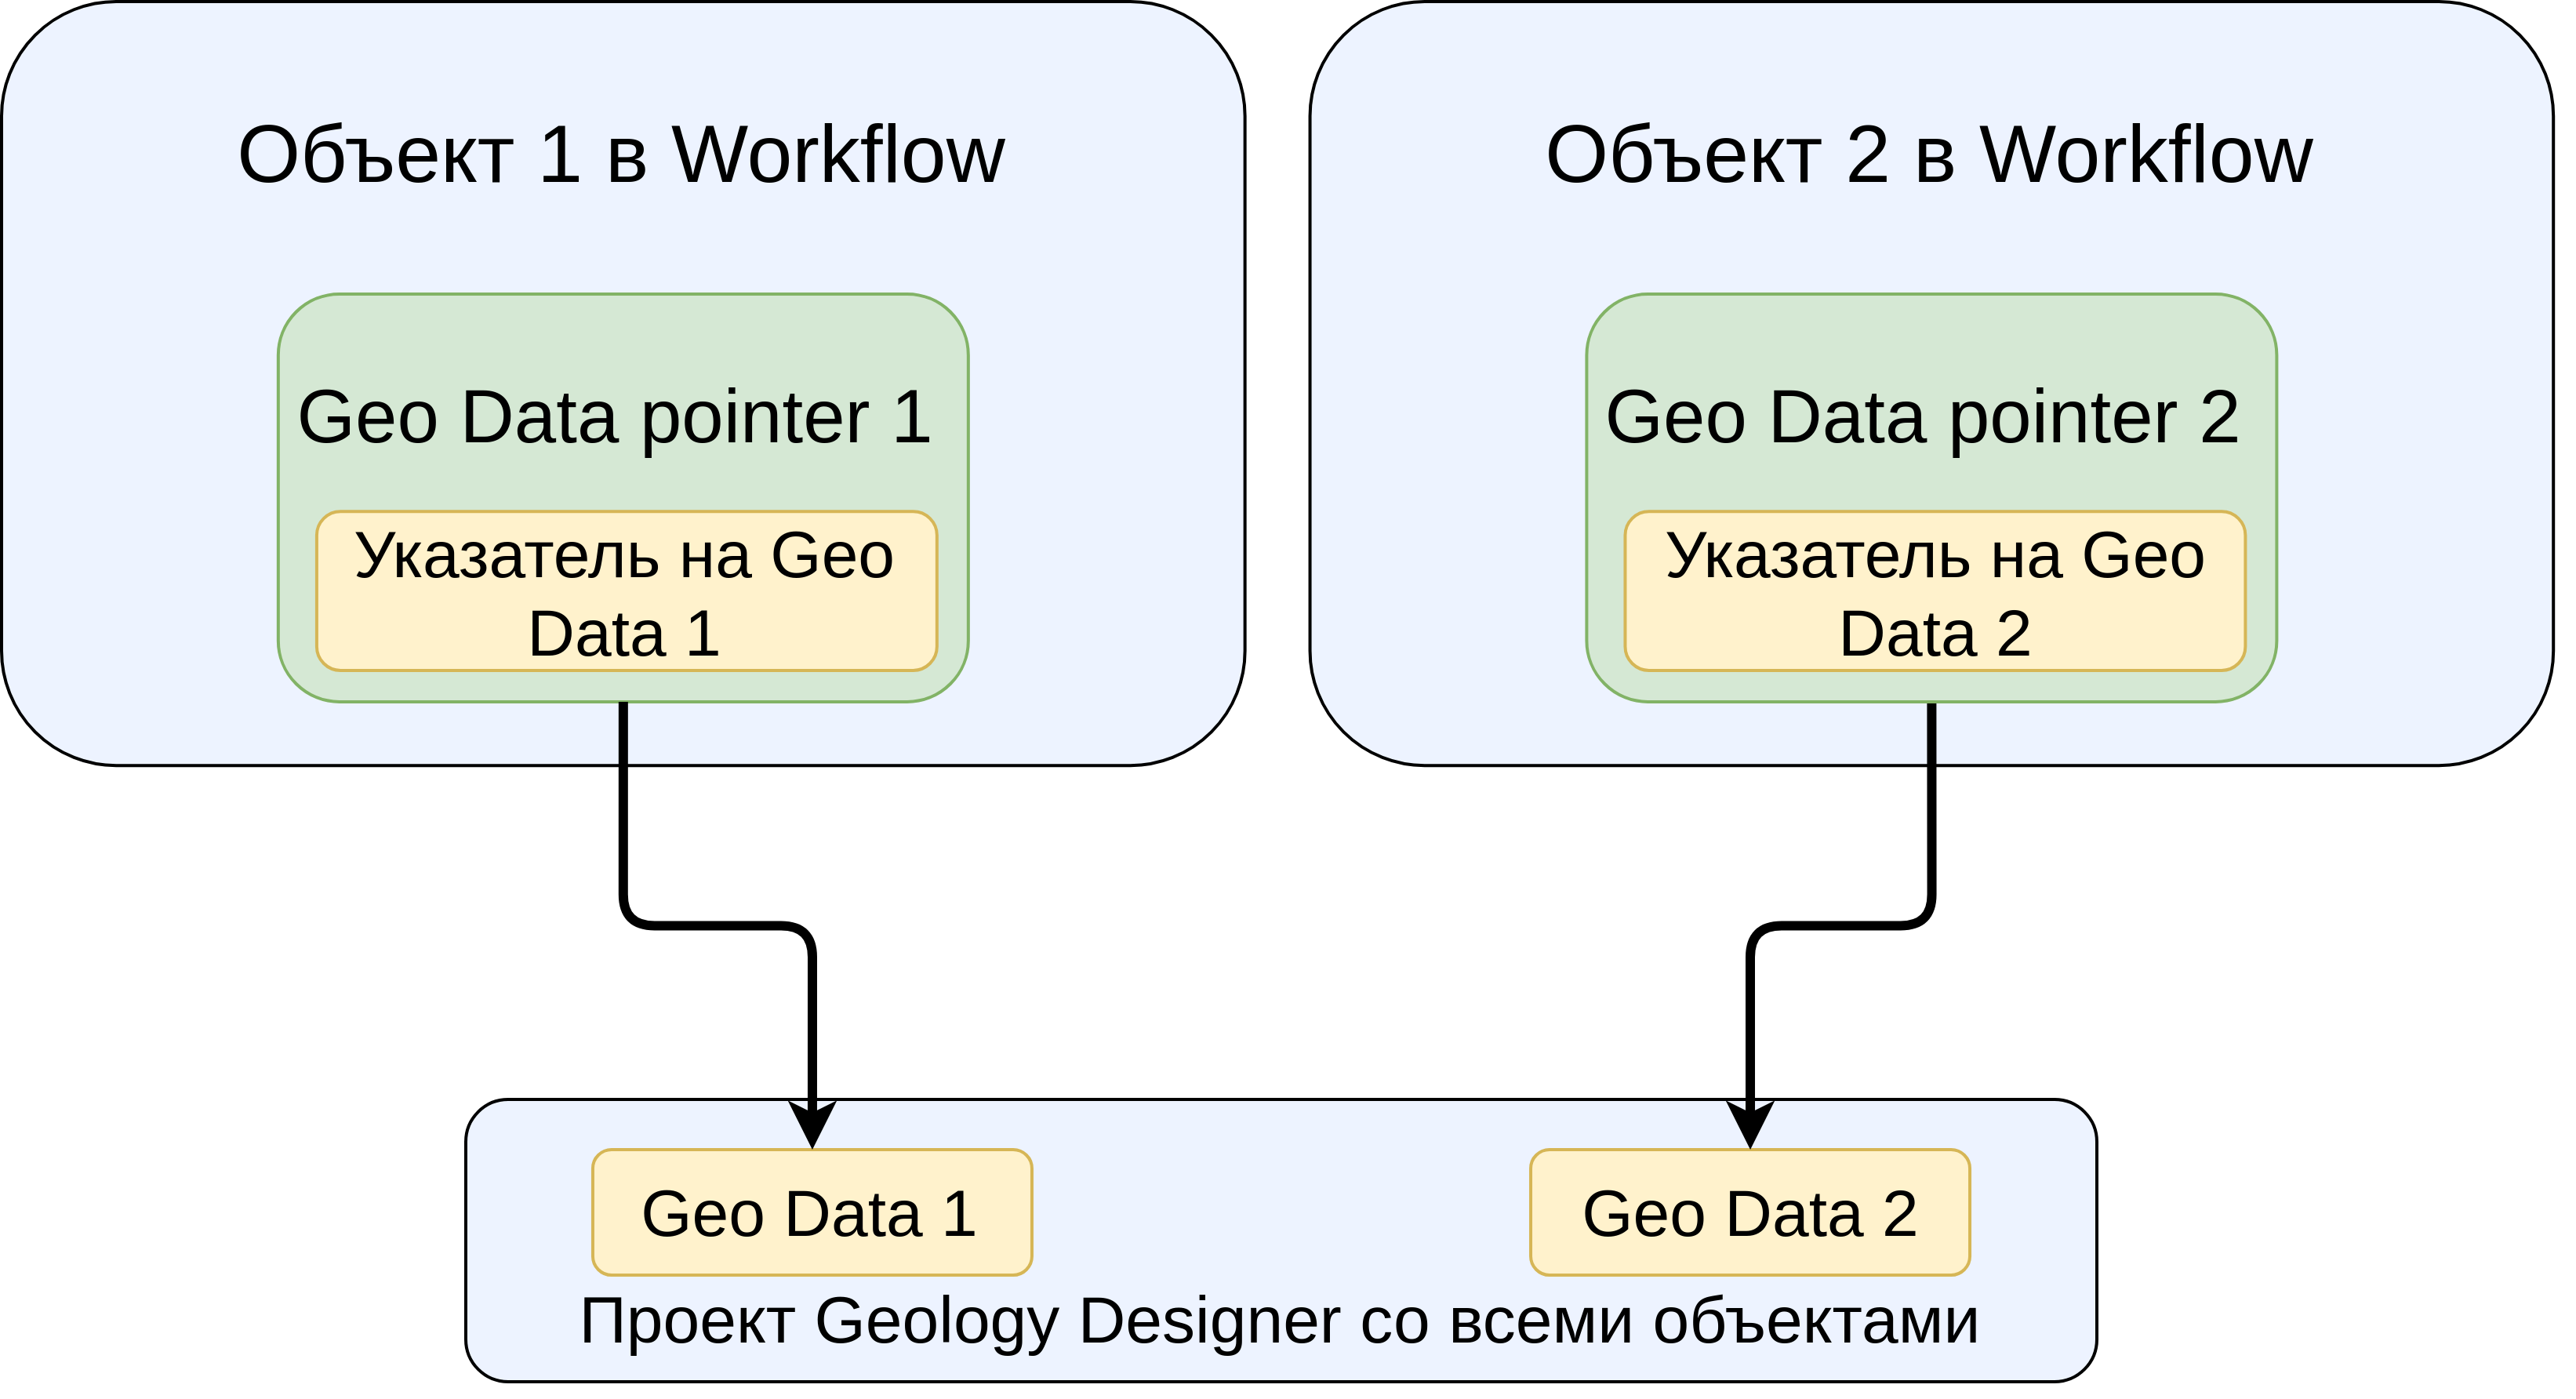
\includegraphics [width=460pt]{pics/object_logic_after.png}}
	\caption{Новая логика хранения объектов в Workflow}
\end{figure}



	
%%	\section{Численный эксперимент}
Из-за измененной логики хранения объектов в \emph{Workflow} возникла необходимость сравнить производительность до и после изменений. Чтобы выяснить насколько приемлимо данное решение поставленной проблемы. 
Для теста был использован проект с 5000 объектами. Были проведены замеры времени обращения к объекту через \emph{Workflow} по следующему сценариям: поиск 5000 различных объектов через \emph{Custom code} и вызов метода \emph{Python}-объекта.

Результаты:
\begin{center}
	\begin{tabular}{|c|c|c|}
		\hline
		& Без \emph{Geo Data pointer} &  C \emph{Geo Data pointer}\\
		\hline
		Время (сек.) & 33.4 & 31.6 \\
		\hline
	\end{tabular}
\end{center}

Из результатов численного эксперимента можно увидеть, что время обращения к объектам существенно не изменилось, что подтверждает корректность нашей реализации и возможность ее внедрения в \emph{Geology Designer}.
	
%%	\section{Заключение}
В результате написания курсовой работы была поддержана корректная работа с объектами в Workflow.

	\newpage
	\begin{thebibliography}{100}
		\bibitem{tNavigator} tNavigator User Guide, \emph{Rock Flow Dynamics, 2021}
		\bibitem{Kalinin_2018} Калинин Н.В, Реализация взаимодействия графического приложения на C++ и языка Python для автоматизации рабочего процесса, \emph{МГУ им. Ломоносова, 2018}
		\bibitem{UUID} RFC 4122, ISO/IEC 9834-8:2005, \emph{IETF, 2005}
		\bibitem{Pybind} \href {https://pybind11.readthedocs.io/en/stable/} {Pybind11 Reference manual}

	\end{thebibliography}


\end{document}
